% This is "sig-alternate.tex" V1.8 June 2007
% This file should be compiled with V2.3 of "sig-alternate.cls" June 2007
%
% This example file demonstrates the use of the 'sig-alternate.cls'
% V2.3 LaTeX2e document class file. It is for those submitting
% articles to ACM Conference Proceedings WHO DO NOT WISH TO
% STRICTLY ADHERE TO THE SIGS (PUBS-BOARD-ENDORSED) STYLE.
% The 'sig-alternate.cls' file will produce a similar-looking,
% albeit, 'tighter' paper resulting in, invariably, fewer pages.
%
% ----------------------------------------------------------------------------------------------------------------
% This .tex file (and associated .cls V2.3) produces:
%       1) The Permission Statement
%       2) The Conference (location) Info information
%       3) The Copyright Line with ACM data
%       4) NO page numbers
%
% as against the acm_proc_article-sp.cls file which
% DOES NOT produce 1) thru' 3) above.
%
% Using 'sig-alternate.cls' you have control, however, from within
% the source .tex file, over both the CopyrightYear
% (defaulted to 200X) and the ACM Copyright Data
% (defaulted to X-XXXXX-XX-X/XX/XX).
% e.g.
% \CopyrightYear{2007} will cause 2007 to appear in the copyright line.
% \crdata{0-12345-67-8/90/12} will cause 0-12345-67-8/90/12 to appear in the copyright line.
%
% ---------------------------------------------------------------------------------------------------------------
% This .tex source is an example which *does* use
% the .bib file (from which the .bbl file % is produced).
% REMEMBER HOWEVER: After having produced the .bbl file,
% and prior to final submission, you *NEED* to 'insert'
% your .bbl file into your source .tex file so as to provide
% ONE 'self-contained' source file.
%
% ================= IF YOU HAVE QUESTIONS =======================
% Questions regarding the SIGS styles, SIGS policies and
% procedures, Conferences etc. should be sent to
% Adrienne Griscti (griscti@acm.org)
%
% Technical questions _only_ to
% Gerald Murray (murray@acm.org)
% ===============================================================
%
% For tracking purposes - this is V1.8 - June 2007

\documentclass{Localization-PaperWriteupDraft}
\usepackage[small,bf]{caption}
\usepackage{caption}
\usepackage{subfig}


\begin{document}
%
% --- Author Metadata here ---
%\conferenceinfo{WOODSTOCK}{'97 El Paso, Texas USA}
%\CopyrightYear{2007} % Allows default copyright year (200X) to be over-ridden - IF NEED BE.
% ACM CoNEXT 2008: the following needs to be over-ridden to include the
% right copyright info
%\crdata{0-12345-67-8/90/01}  % Allows default copyright data (0-89791-88-6/97/05) to be over-ridden - IF NEED BE.
% --- End of Author Metadata ---

\title{Learning to Localize}
\subtitle{[Draft - v2.0 - Jun 8, 2011 - changes made in the 'Introduction' and 'Experiment Methodology' ]}
%
% You need the command \numberofauthors to handle the 'placement
% and alignment' of the authors beneath the title.
%
% For aesthetic reasons, we recommend 'three authors at a time'
% i.e. three 'name/affiliation blocks' be placed beneath the title.
%
% NOTE: You are NOT restricted in how many 'rows' of
% "name/affiliations" may appear. We just ask that you restrict
% the number of 'columns' to three.
%
% Because of the available 'opening page real-estate'
% we ask you to refrain from putting more than six authors
% (two rows with three columns) beneath the article title.
% More than six makes the first-page appear very cluttered indeed.
%
% Use the \alignauthor commands to handle the names
% and affiliations for an 'aesthetic maximum' of six authors.
% Add names, affiliations, addresses for
% the seventh etc. author(s) as the argument for the
% \additionalauthors command.
% These 'additional authors' will be output/set for you
% without further effort on your part as the last section in
% the body of your article BEFORE References or any Appendices.

\numberofauthors{3} %  in this sample file, there are a *total*
% of EIGHT authors. SIX appear on the 'first-page' (for formatting
% reasons) and the remaining two appear in the \additionalauthors section.
%
\author{
% You can go ahead and credit any number of authors here,
% e.g. one 'row of three' or two rows (consisting of one row of three
% and a second row of one, two or three).
%
% The command \alignauthor (no curly braces needed) should
% precede each author name, affiliation/snail-mail address and
% e-mail address. Additionally, tag each line of
% affiliation/address with \affaddr, and tag the
% e-mail address with \email.
%
% 1st. author
\alignauthor
AG\\
%Abhishek Goswami\\
       \affaddr{Computer Science}\\
       \affaddr{Stony Brook University}\\
       \email{agoswami@cs.sunysb.edu}
% 2nd. author
\alignauthor
SD\\
%Samir Das\\
       \affaddr{Computer Science}\\
       \affaddr{Stony Brook University}\\
       \email{samir@cs.sunysb.edu}
% 3rd. author
\alignauthor 
LO\\
%Luis Ortiz\\
       \affaddr{Computer Science}\\
       \affaddr{Stony Brook University}\\
       \email{leortiz@cs.sunysb.edu}
}

\date{03 June 2011}

\maketitle
\begin{abstract}

We consider the problem of localizing a wireless client in an
indoor environment based on the signal strength of its transmitted
packets as received on stationary sniffers or access points.

Current state-of-the art indoor localization techniques have the
drawback that they rely extensively on a `training phase'.  This
`training' is a labor intensive process and must be done for
each target-area under consideration for various device types.
This clearly does not scale for large target areas. The
introduction of unmodeled hardware with heterogeneous
power-levels etc further reduces the accuracy of these
techniques.

We propose a solution in which we model the received signal
strength as a Gaussian Mixture Model (GMM). We use expectation
maximization to find the parameters of our GMM. We can now give
a location fix for a transmitting device based on the maximum
likelihood estimate. This way, we not only avoid the costly
`training phase' but also make our location estimates much more
robust in the face of various form of heterogeneity and time
varying phenomena.  We present our results on two different
indoor testbeds (CEWIT and Computer Science Buildings in Stony
Brook University) with multiple WiFi devices (iphones,
android, laptops, netbooks). We demonstrate that the
accuracy is at par with state-of-the-art techniques but
without requiring any training.

\end{abstract}

% A category with the (minimum) three required fields
\category{H.4}{Information Systems Applications}{Miscellaneous}
%A category including the fourth, optional field follows...
\category{D.2.8}{Software Engineering}{Metrics}[complexity measures, performance measures]

\terms{Delphi theory}

\keywords{ACM proceedings, \LaTeX, text tagging}

\section{Introduction}
\label{sec:introduction}

The increasing use of wireless networking has fueled the need for location-aware pervasive computing applications in indoor environments. Traditional GPS-based techniques have problems working indoor which make them unattractive for such fine-grained indoor localization. On the other hand, indoor wireless LAN (WLAN) technologies, which have been enthusiastically and widely adopted in enterprises and homes, give us interesting features like Received Signal Strength(RSS), Angle of Arrival(AoA) etc for robust location estimation. Received signal strength (RSS) is particularly interesting because current commercial hardware can be used to extract the signal strength of wireless frames being transmitted by a Wi-Fi device. 

Several techniques [x, y, x] have demonstrated the viability of using the RSS metric for location estimation.   It is interesting to note here that most of these location-estimation systems can essentially be categorized in two distinct ways : a client-based approach [p, q, r] and an infrastructure-based approach [a, b, c]. In the client-based approach, the client device measures the signal strength as seen by it from various AP(Access Point). This information is used to locate the client. In the infrastructure-based approach, the network administrator can use simple sniffing devices (or APs masquerading as sniffers) to monitor clients and extract the RSS from the tx-client.  This sniffed information is used to locate the client. Considering ease of management, provisioning, security, deployment,  maintenance etc, the infrastructure-based model seems alluring for large-scale deployments, especially if building and maintaining the model can be automated. Moreover, such techniques perform location estimation without requiring hardware and/or software changes on the client device, which make them particularly attractive.

Most of the existing solutions for WLAN location estimation work in two phases. The first phase is a pre-deployment 'offline phase' aimed at building detailed RF maps or RF propagation models based on a survey of the target location. The second phase is an 'online phase' of location estimation, where a localization algorithm is used to give a location estimate for an observed set of signal strength measurements. All such techniques suffer from three major drawbacks that serve as the motivation for this present work :

First, the WiFi hardware variance problem : the device used during the 'offline phase' may differ from the target device in the 'online phase'. Unmodeled hardware devices operating at different power-levels can introduce significant variations in the signal patterns between the training device and the target device. This adversely affects the accuracy of location estimation. Experiments described later in this paper indicate how hardware variance between four common commodity WiFi devices can significantly degrade the positional accuracy of two commonly used localization algorithms. 

Second, the 'offline phase' requires an extensive pre-deployment effort which usually involves labor-intensive sampling of signal strength values at discretized locations in the target space. Again, through experiments we show that location accuracy depends significantly on the granularity of discretization. An 'offline phase'  which uses a coarse-grained discretization of the target area gives poorer accuracy estimates compared to the corresponding fine-grained discretization. However, finer discretization involves higher pre-deployment effort.

Third, static models built during the 'offline phase' can substantially reduce the accuracy of location estimates in the presence of time varying phenomena like movement of people inside the building, changing environmental and occupancy conditions etc. The heavy pre-deployment effort makes such models difficult to maintain and update. 

In this work, we propose a novel indoor localization algorithm, GEM, that tries to leverage the infrastructure based model of location determination systems while eliminating any pre-deployment effort. Packet transmissions made by a client are received on stationary sniffers or access points which extract the signal strength and mac-id of the client, and report this information to a central localization server. Using this information, GEM builds a model for that device and gives a location estimate based on the model. 

GEM provides several key benefits by eliminating the 'offline phase' . First, by building a model for each target device effectively addresses the hardware variance problem. Thus GEM can be used across heterogeneous devices, each operating at different power levels.  Second, no pre-deployment effort makes GEM particularly attractive for large target spaces like malls, office spaces etc  Third, GEM is an online algorithm : the model parameters get updated and modified based on real-time signal strength observations. . As such, GEM is able to adapt to dynamic changes in the target space.

Our results of deploying GEM in two different office buildings are promising. We specifically note that when measurements made using one device are used to localize a different device,  GEM is seen to perform better that RF signal map based techniques like RADAR[x] and Probabilistic[y]

\section{Related Work}
\label{sec:relatedwork}


Some calibration-free techniques have been proposed \cite{Moraes:2006:CWL:1164783.1164799}
\cite{Gwon:2004:ECC:1023783.1023786} \cite{Lim:2010:ZIL:1741400.1741464} etc. The objective of such techniques is
to automate the effect of wireless physical characteristics on RSS
measurements and make them responsive to environmental dynamics like
temperature and humidity variations, furniture variation, human mobility
etc. This is usually done by having reference Access Points (or
sniffers) deployed in the target space and then measuring RSS between
the 802.11 APs and also between a client and its neighbouring APs (or
sniffers). In \cite{Moraes:2006:CWL:1164783.1164799} Moares et al use an indoor signal propagation model to generate a 
{\it radio propagation map (RPM)} at each sniffer. Thereafter they use
RSS measurements between the sniffers and a reference Access Point(AP)
to reconstruct the RPM, either periodically or when there are
significant variations of RSS values. In \cite{Lim:2010:ZIL:1741400.1741464} Lim et al. use
the on-line RSS measurements to create a mapping between the RSS measure
and the actual geographical distance.

Such techniques are essentially modelled to capture real-time changes in
the environmental dynamics of the target space. But they do not model variations in client
hardware and transmission power which can significantly degrade the
positional accuracy of RSS based Wi-Fi localization schemes.

In \cite{Tsui:2009:ULS:1741410.1741596} Tsui et al. also observe that hardware variance can
significantly degrade the positional accuracy of RSS-based Wi-Fi
localization systems. Infact they note that the hardware variance
problem is not limited to differences in the WiFi chipsets used by
training and tracking devices but also occurs when the same Wi-Fi
chipsets are connected to different antenna types and/or packaged in
different encapsulation materials. The authors stick to the
{\it online}-training and {\it offline} location-determination model
but add an intermediate online-adjustment phase . In this intermediate
phase they use unsupervised learning methods to construct a signal
transformation function between the training device and a new tracked
device.

In \cite{Tao:2003:WLL:941311.941314} Tao et al. have an interesting take on unmodelled-hardware and
transmission power variations being effected by a transmitting client.
They also stick to the {\it online}-training and {\it offline}
location-determination model. However, they observe that RSS is linearly proportional to transmission power.
Thus the difference in received signal strengths between a pair of
sniffer devices would not vary dramatically as the transmission power
of a client device changes. Based on the difference in signal strength between every pair
of sniffers, they suggest a weighted heuristic to estimate a
location-fix for a given target RSS fingerprint. With such a
`difference' based approach, we can no longer assume that the sniffers
are independent. Thus, we are restricted to the use of a heuristic in
this model. However, the observation that RSS is linearly proportional to transmission power
is very interesting. Infact, we use this observation in building our
model.

The major contribution of this work is to develop an algorithm that does
not rely on training data. Instead, the algorithm can learn the
parameters of the model from real-time transmissions being made by a
Tx-client. Thus it can adapt to variations in transmit power across
heterogeneous devices which makes it particularly suitable for
server-side localization techniques. Plus this model can also factor in
real-time changes in the environmental dynamics of the target space. 

\section{Wireless Characteristics}
\label{sec:wirelesscharacteristics}

\begin{figure*}
\begin{minipage}{0.3\textwidth}
\includegraphics[width=1\textwidth]{Figs4Paper/GaussianDistr/gaussian.eps}
\caption{The distribution of RSS observed on a sniffer}
\label{fig:distribution}
\end{minipage}\quad %
\begin{minipage}{0.3\textwidth}%
\includegraphics[width=1\textwidth]{Figs4Paper/TxPower/Tx_PowerLevels.eps}
\caption{RSS as a function of the Tx-power of a device.}
\label{fig:txpower}
\end{minipage}\quad%
\begin{minipage}{0.3\textwidth}%
\includegraphics[width=1\textwidth]{Figs4Paper/gmm.eps}
\caption{The GMM for our problem}
\label{fig:gmm}
\end{minipage}%
\end{figure*}


% \begin{figure*}[h!]
% \begin{minipage}{0.52\textwidth}
% %\subfloat[big]{\label{subfig:a}\includegraphics[width=1\textwidth]{Figs/gaussian.eps}} \\%
% %\subfloat[big2]{\label{subfig:a}\includegraphics[width=1\textwidth]{Figs/gaussian.eps}}%
% 
% \includegraphics[width=1\textwidth]{Figs/gaussian.eps}
% \caption{first minipage}
% \end{minipage}\quad %
% \begin{minipage}{0.33\textwidth}%
% \subfloat[small]{\label{subfig:b}\includegraphics[width=1\textwidth]{Figs/gaussian.eps}}\\%
% \subfloat[small]{\label{subfig:c}\includegraphics[width=1\textwidth]{Figs/gaussian.eps}}%
% \caption{second minipage}
% \end{minipage}%


 %\label{fig:diamond_lattice}
 %\caption{Face-Center-Cubic - \ref{subfig:a}  \ref{subfig:b} \ref{subfig:c} }

%\end{figure*}



% \begin{figure}[h!]
%   \centering
%     \epsfig{file=Figs/gaussian.eps, height=1.5in, width=2.5in}
%   \caption{ Received Signal Strength at a sniffer from a laptop operating at a fixed power-level }
%   \label{fig:gaussian}
% \end{figure}
% 
% \begin{figure}[h!]
% \centering
%   \epsfig{file=Figs/Tx_PowerLevels.eps, height=1.5in, width=2.5in}
%   \caption{Signal strength readings from three different receivers of a signal from a signal transmitter, with the transmitter varying it Tx-Power}
%   \label{fig:txpower}
% \end{figure}

Our system is based on the 802.11 wireless networking protocol, which is
inexpensive and widely deployed in enterprise offices and academic
campuses. 802.11 uses 11 channels in the ISM band. Signal
propagation in this band is complex and in this section, we identify the different
causes of variation in the wireless channel quality and how we factor
them into our model. Our approach is server-based, where we capture
client packets using sniffers. As such, we are mainly concerned with the
variations that affect the Received Signal Strength (RSS) on the
sniffer. In this section, experimentally validate two observations that have been made previously
in wireless-localization literature. We model our problem around these
two observations. 

\subsection{Distribution of Signal Strength}
\label{subsec:distributionofsignalstrength}

Figure \ref{fig:distribution} shows the distribution of Received Signal
Strength values observed by a sniffer located a fixed distance apart
from a transmitting client. The Tx-client is a Dell laptop having a
Ubiquiti XR2 wireless card and is using a fixed power-level for wireless
transmissions. 

We observe that the Signal Strength distribution is roughly Gaussian. In
\cite{Tao:2003:WLL:941311.941314} et al also make similar observations.
\cite{Haeberlen:2004:PRL:1023720.1023728} \cite{Moraes:2006:CWL:1164783.1164799} etc also model signal intensity
as a normal distribution.

\subsection{Transmission Power}
\label{subsec:transmissionpower}

Figure \ref{fig:txpower} shows how the observed signal strength changes
as the transmission power is varied. Our experiments validate the
observations made in \cite{Tao:2003:WLL:941311.941314} by Tao et al in that the observed
signal strength is linearly proportional to the transmission power.

\section{Problem Formulation}
\label{sec:problemformulation}

The Gaussian Mixture Model is a simple linear superposition of Gaussian components, aimed at providing a richer class of density models than the single Gaussian. We now formulate our problem as a Gaussian mixture in terms of discrete latent variables. 

% \begin{figure}[!ht]
% 	\centering
% 		\epsfig{file=Figs/gmm.eps, height=1.5in, width=2.5in}
% 	\caption{Gaussian Mixture Model}
% 	\label{fig:gmm}
% \end{figure}

\subsection{Latent Variables for Target Locations and Power Levels}
\label{subsec:latentvariablesfortargetlocationsandpowerlevels}

We introduce a J-dimensional binary random variable {\bf x} representing possible target locations. {\bf x} has a 1-of-J representation in which a particular element $x_{j}$ is equal to one and all other elements are equal to 0. The values of $x_{j}$ therefore satisfy $x_{j} \in$ \{0,1\} and $\sum_{j} x_{j} = 1$. Thus we see that there are J possible states for the vector {\bf x} \\

The probability distribution over {\bf x} can be specified as a multinomial 

\begin{align}
 p(x_{j} = 1) = \upsilon_{j}
\end{align}

where the parameters $\{\upsilon_{j}\}$ must satisfy
\begin{align}
0 \le \upsilon_{j} \le 1 \ and \ \sum_{j=0}^{J} \upsilon_{j} = 1
\end{align}

Similarly, let us introduce a K-dimensional binary random variable {\bf z} representing Power Levels. {\bf z} has a 1-of-K representation in which a particular element $z_{k}$ is equal to one and all other elements are equal to 0. The values of $z_{k}$ therefore satisfy $z_{k} \in$ \{0,1\} and $\sum_{k} z_{k} = 1$. Vector {\bf z} has K possible states.

The distribution over {\bf z} is specified as a multinomial 
\begin{align}
p(z_{k} = 1) = \tau_{k}
\end{align}

where the parameters $\{\tau_{k}\}$ must satisfy
\begin{align}
0 \le \tau_{k} \le 1 \ and \  \sum_{k=0}^{K} \tau_{k} = 1
\end{align}

\subsection{Constructing the distribution over the observed signal strengths}
\label{subsec:constructingthedistributionovertheobservedsignalstrengths}

Let {\bf s} be the N-dimensional vector representing the signal strengths observed by the N sniffers placed in the area. 

Using the chain rule of probability, we can now define the joint distribution $p( {\bf s}, {\bf x}, {\bf z})$ in terms of the distribution $p( {\bf x}, {\bf z})$ and the conditional distribution $p( {\bf s} | {\bf x}, {\bf z})$, corresponding to the graphical model in Figure \ref{fig:gmm}.

\begin{align}
p( {\bf s}, {\bf x}, {\bf z}) &= p( {\bf x}, {\bf z}) p( {\bf s} | {\bf x}, {\bf z}) 
\end{align}

Moreover {\bf x} and {\bf z} are independent random variables. So we have

\begin{align}
p( {\bf s}, {\bf x}, {\bf z}) &= p( {\bf x}, {\bf z}) p( {\bf s} | {\bf x}, {\bf z}) \nonumber \\
&= p({\bf x})p({\bf z})p( {\bf s} | {\bf x}, {\bf z}) \label{eqn:joint_distribution}
\end{align}

Equation \ref{eqn:joint_distribution} gives us the joint distribution of $ p( {\bf s}, {\bf x}, {\bf z}) $. The marginal distribution of {\bf s} is then obtained by summing the joint distribution over all possible states of {\bf x} and {\bf z} to give the following probabilistic model :

\begin{align}
p( {\bf s}) & = \sum_{\bf x}\sum_{\bf z} p({\bf x})p({\bf z})p({\bf s}|{\bf x}, {\bf z}) \label{eqn:marginal_distribution1}
\end{align}

\subsubsection{Independence of Sniffers}
\label{subsubsec:independenceofsniffers}

We assume the sniffers are independent. This assumption is justified in our model because our sniffers are passive nodes responsible for capturing wireless packets. They have no interaction with each other. 

Thus, the term $p( {\bf s} | {\bf x}, {\bf z})$ in equation
\ref{eqn:marginal_distribution1} can be simplified as

\begin{align}
p( {\bf s} | {\bf x}, {\bf z}) & = \prod_{i=1}^N p({s_{i}}|{\bf x}, {\bf
		z}) \label{eqn:conditional_distribution1}
\end{align}

Moreover, from the observations made about Signal Strength variations in
Section \ref{subsec:distributionofsignalstrength} above, the distribution of signal strength
can be modelled as a Gaussian determined by the (location, power-level) pair. 

That is 

\begin{align}
s_{i} | ({x_{j}}, {z_{k}})  \sim  gaussian (\mu_{i \ (j,k)} \ , \sigma_{i \ (j,k)})
\end{align}

This lends simplicity to our model since the term $p( {\bf s} | {\bf x}, {\bf z})$ in equation
\ref{eqn:conditional_distribution1} can be further simplified as 

\begin{align}
p( {\bf s} | {\bf x}, {\bf z}) & =  \sum_{j=1}^J \sum_{k=1}^K (
		\prod_{i=1}^N {\it \mathcal  N}[ {s_{i}} | \mu_{i \ (j,k)} \ ,
		\sigma_{i \ (j,k)}] ) \label{eqn:conditional_distribution2}
\end{align}

\subsection{Model Parameters}
\label{subsec:modelparameters}

Putting equation \ref{eqn:marginal_distribution1} and equation
\ref{eqn:conditional_distribution2} together we get the distribution of
{\bf s} as

\begin{align}
p( {\bf s}) &= \sum_{j=1}^J \sum_{k=1}^K ( \upsilon_{j} \tau_{k} \prod_{i=1}^N {\it \mathcal  N}[ {s_{i}} | \mu_{i \ (j,k)} \ ,
		\sigma_{i \ (j,k)}] )
\end{align}

Thus we have modelled the marginal distribution of {\bf s} as a Gaussian
mixture with target locations and power levels as our latent variables. The parameters of our model are 
\begin{align}
{\bf \theta} = \left( \upsilon_{j} , \tau_{k}, (\mu_{i \ (j,k)} , \sigma_{i \ (j,k)} )\right)
\end{align}
where $j\in\{1,...J\},\ k \in\{1,...K\}$ and $i\in \{1,...N\}$. We now use the  Expectation Maximization(EM) algorithm to estimate the parameters of our model.

\section{EM Algorithm}
\label{sec:emalgorithm}

An elegant and powerful method for finding maximum likelihood solutions
for models with latent variables is the Expectation Maximization(EM)
	algorithm. The EM algorithm is an iterative process through two
	steps: an expectation step(E-step) and a maximization step(M-step). During the iterations, a sequence of model parameters ${\bf \theta^{0}}$
, ${\bf \theta^{1}}$, ...., ${\bf \theta^{*}}$ is generated where ${\bf \theta^{0}}$ is the initial parameter and ${\bf \theta^{*}}$ is the converged parameter obtained when the algorithm terminates.

\subsection{E-step}
\label{subsec:estep}

Suppose we have a data set of observations  ${\bf \overline{S}}$ = \{
${\bf {s}}^{0}$, ${\bf {s}}^{1}$, ....,${\bf {s}}^{M}$\}. The E-step
corresponds to finding the expected value of the hidden component ({\bf
		x} and {\bf z}) values given the observed data  ${\bf \overline{S}}$ and the current parameter estimates.

Using this observation set and the current parameter estimates, we find out the posterior probabilities (or responsibilities) as follows. 

For each observation ${\bf {s}}^{l}$
\begin{align}
& \pi_{({x_{j}}, {z_{k}})}^{l}  = p({x_{j}} = 1, {z_{k}} = 1 | {\bf{s}}^{l}) \\ 
& = \frac { p({x_{j}} = 1)p({z_{k}} = 1)p( {\bf {s}}^{l} | {x_{j}} = 1, {z_{k}} = 1)} {\ \sum_{p=1}^J \ \sum_{q=1}^{K} p({x_{p}} = 1) p({z_{q}} = 1) p( {\bf {s}}^{l} | {x_{p}} = 1, {z_{q}} = 1)} \nonumber \\
& = \frac { \upsilon_{j} \ \tau_{k} N({\bf {s}}^{l} | {\bf {\mu}}_{j,k}, {\bf {\sigma}}_{j,k})} {\sum_{p=1}^J \sum_{q=1}^K \left[\upsilon_{p} \tau_{q} N({\bf {s}}^{l} | {\bf {\mu}}_{p,q}, {\bf {\sigma}}_{p,q})\right] }
\end{align}

The posterior probability value $\pi_{({x_{j}}, {z_{k}})}^{l}$ can be viewed as the {\it responsibility} that component $({x_{j}}, {z_{k}})$ takes for explaining observation ${\bf {s}}^{l}$. We find out this measure of responsibility for each observation in our data set ${\bf \overline{S}}$.

\subsection{M-step}
\label{subsec:mstep}

The M-step of the algorithm corresponds to maximizing the likelihood of
the observed data. This leads us to re-estimating the parameters for the next iteration based on the posterior probabilities calculated in the expectation step of the algorithm.
\begin{align}
\upsilon_{j} = \frac { \sum_{l=1}^{M} \ \sum_{k} \pi_{({x_{j}}, {z_{k}})}^{l}} {M}
\end{align}

\begin{align}
\tau_{k} = \frac { \sum_{l=1}^{M} \ \sum_{j} \pi_{({x_{j}}, {z_{k}})}^{l}} {M}
\end{align}

\begin{align}
\mu_{i \ (j,k)} = \frac  { \sum_{l=1}^{M} \pi_{({x_{j}}, {z_{k}})}^{l} s_{i}^{l}} {N_{j,k}}
\end{align}

where we have defined 
\begin{align}
{N_{j,k}} = \sum_{l=1}^{M} \pi_{({x_{j}}, {z_{k}})}^{l}
\end{align}


The variance parameter can also be updated accordingly.

\subsection{Convergence of Log Likelihood}
\label{subsec:convergenceofloglikelihood}

Each update of the parameters resulting from an E-step followed by an
M-step is guaranteed to increase the log likelihood function. The algorithm is deemed to have converged when the change in the log likelihood function falls below a threshold.

\begin{align}
\ln p({\bf \overline{S}} | {\bf \theta}) &= \sum_{l=1}^{M} \ln \left\{
\sum_{j=1}^J \sum_{k=1}^K \upsilon_{j} \tau_{k} \mathcal N ({{\bf {s}}^{l}} | {{\bf {\mu}}_{j,k}}, {{\bf \sigma}_{j,k}})\right\} 
\end{align}

\subsection{Handling Identifiability in our Model}
\label{subsec:handlingidentifiabilityinourmodel}

In \cite{Bishop:2006:PRM:1162264} Bishop et al discuss the problem of {\it
identifiability} associated with assigning P sets of parameters to P
components. The problem occurs because there are P! ways of assigning P
sets of parameters to P components. 

In our case each component can be represented as a (location,
power-level ) pair. We handle the problem of identifiability as follows :

\subsubsection{Indoor Radio Propagation Model}
\label{subsubsec:indoorradiopropagationmodel}

The indoor radio propagation model is represented as
\begin{align}
P_{Rx} = P_{0} - 10n\log\left(\frac {\it d} {\it d_{0}}\right) 
\end{align}

\noindent
where $P_{0}$ is the received signal strength at a distance $d_{0}$ from the
emitter. $P_{Rx}$ is the signal strength($s_{i}$) seen by receiver for a
transmitter located at a distance {\it d} away from it. {\it n} is a
parameter which models the behaviour of the environment. This formula
effectively initializes the components representing different locations
on the map.

To initialize k components (say) which have a common location but vary in
power-level, we make use of the observations made in Section
\ref{subsec:transmissionpower} which show that the observed signal strength is linearly proportional to the transmission power. 
Thus, once the formula above gives us the signal value for
a specific location, we extrapolate the value linearly to initialize
each of the k components for that location 

In our experiments, we set n = 2. The corresponding signal strength was
used to initialize the means ($\mu_{j, k}$). The standard deviation
($\sigma_{j, k}$) was initialized to
5 (and kept fixed to reduce computation time). As subsequent results
show, a value of k = 45 is sufficient to hit a constant average error
distance.

\subsection{Final Location Estimate}
\label{subsec:finallocationestimate}

\begin{figure*}
	\centering
		\subfloat[CEWIT]{\includegraphics[height=2.5in, width=2in]{Figs4Paper/CEWIT/CEWIT-Map1.eps}} \quad \quad
		\subfloat[CSD]{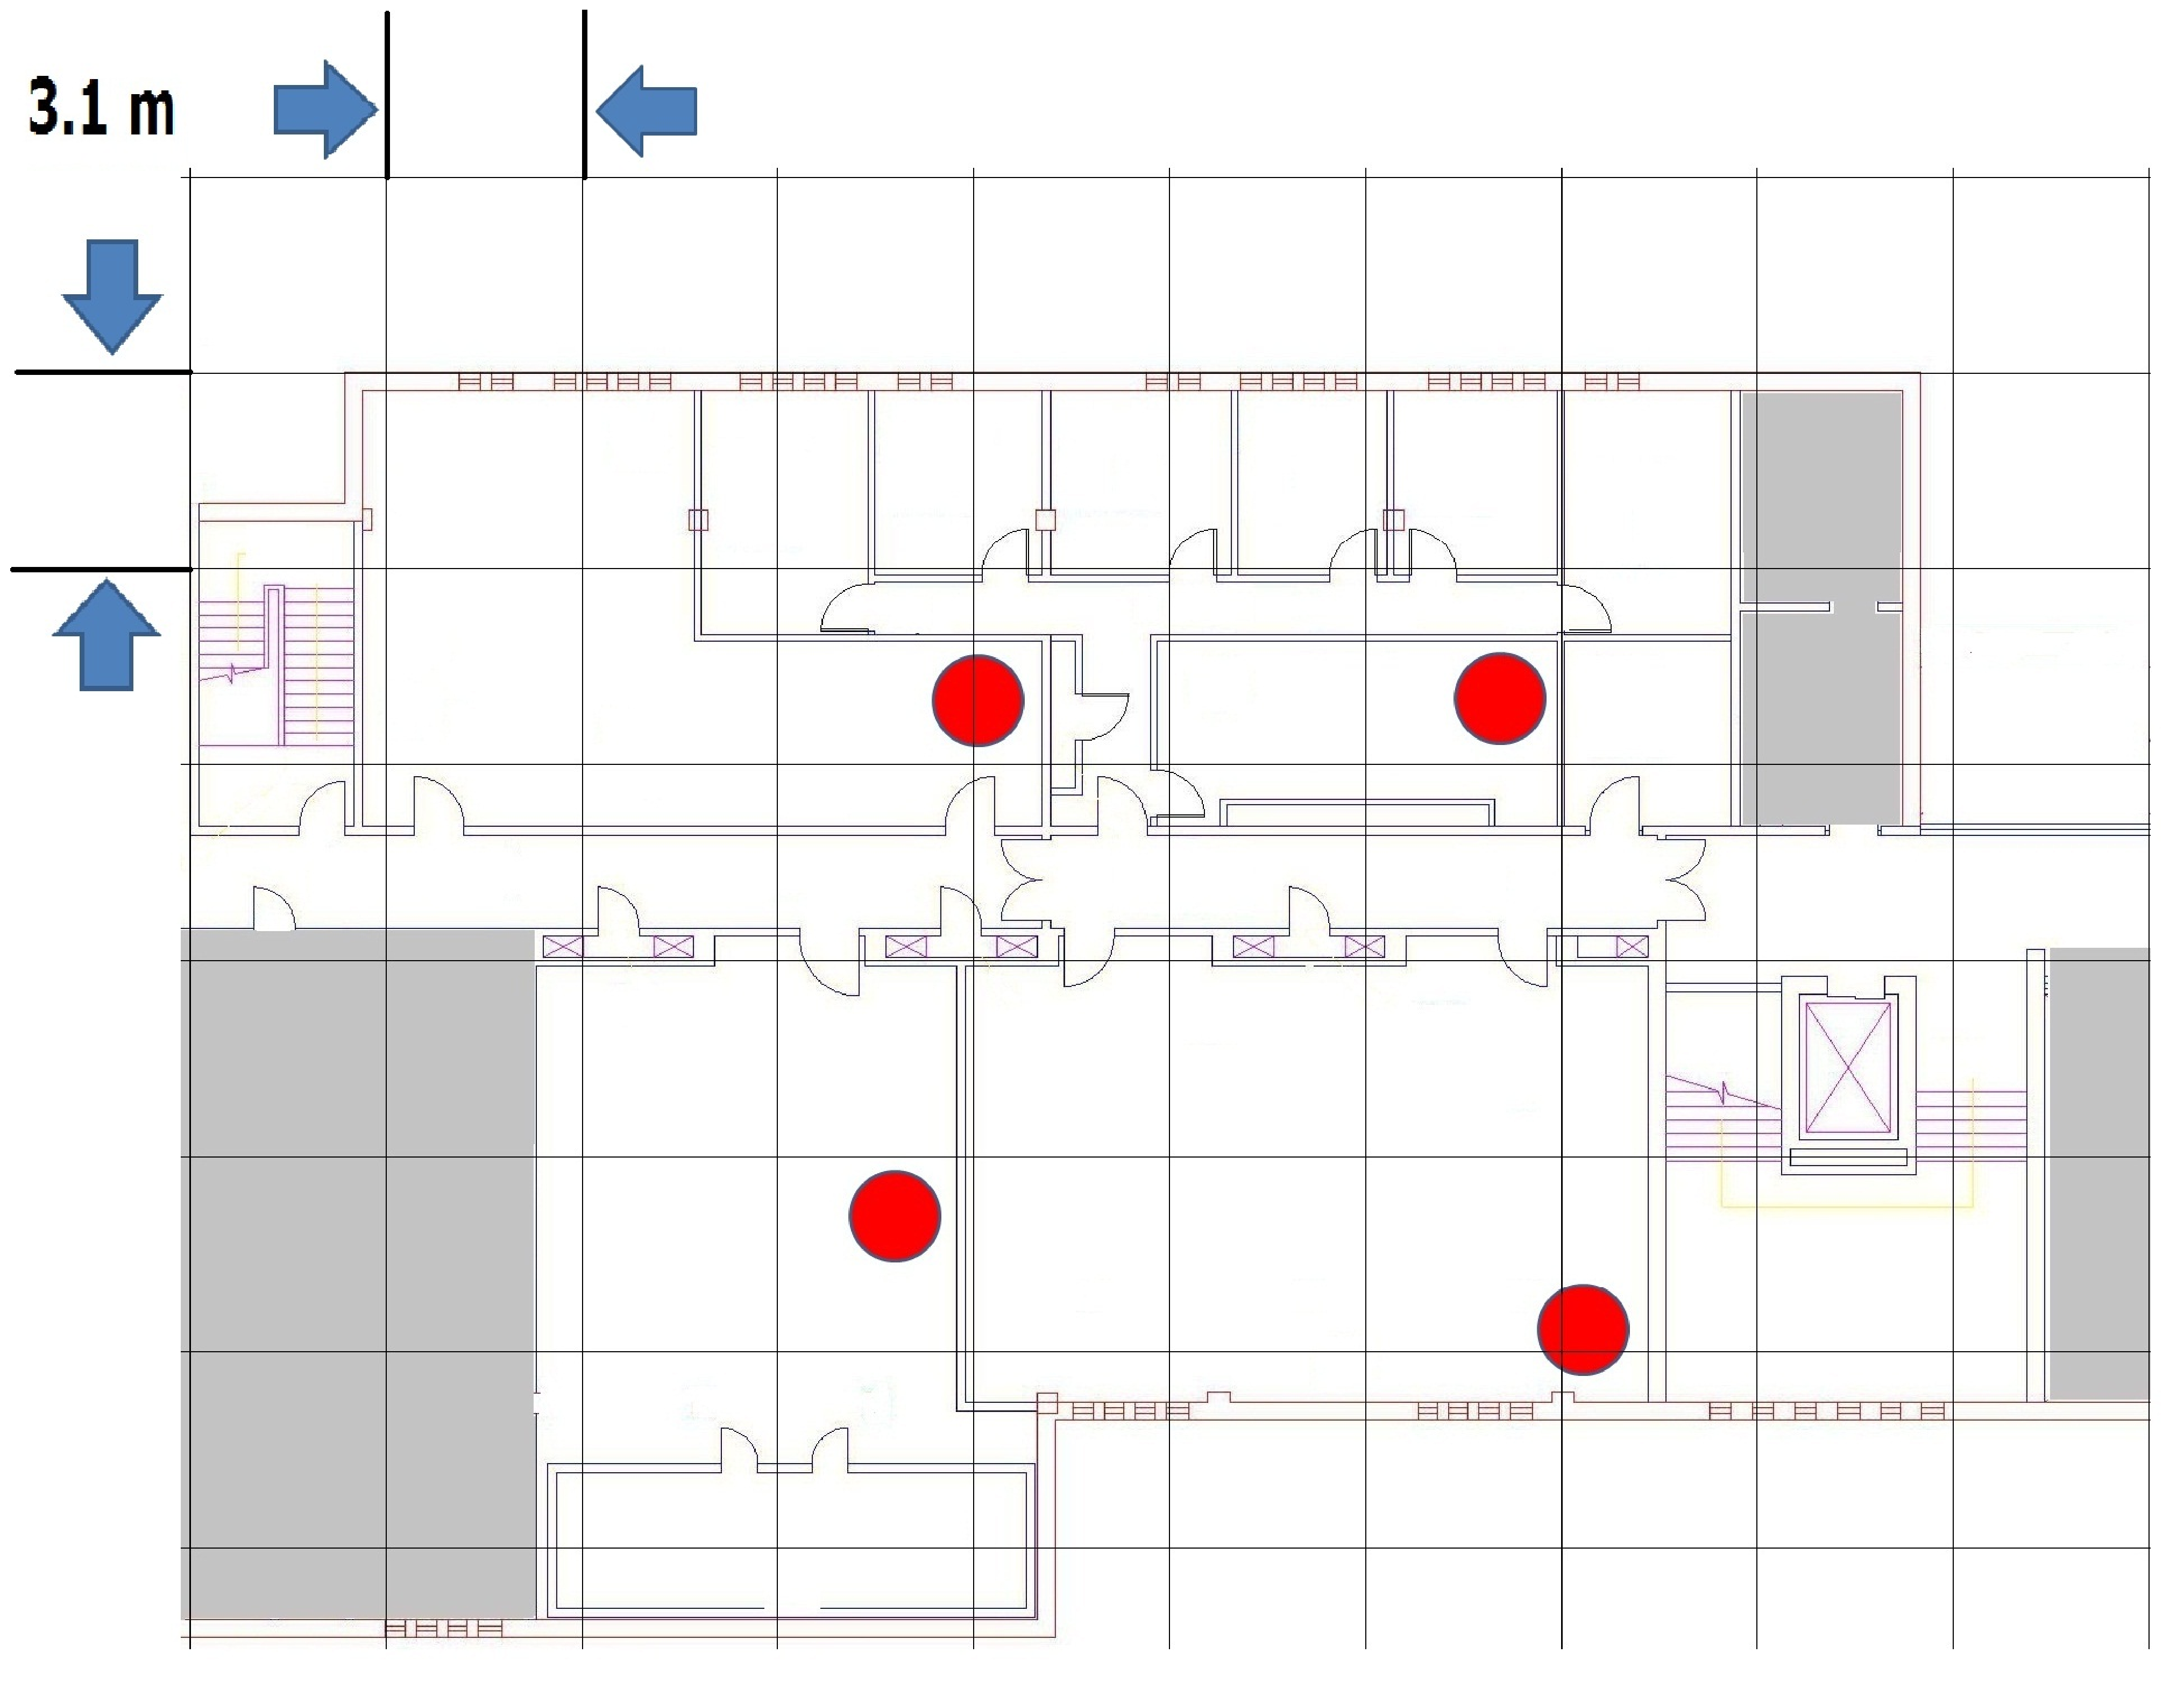
\includegraphics[height=1.5in, width=2.5in]{Figs4Paper/CSD/CSD-Map1.eps}}
	\caption{Number of power levels v/s Avg Error distance}
	\label{fig:powerlevelsvserrordistance}
\end{figure*}

% \begin{figure}
% \centering
%   \epsfig{file=Figs4Paper/CEWIT/CEWIT-Map1.eps, height=2.5in, width=2in}
%   \caption{Map of the CS Dept Building where experiments were conducted}
%   \label{fig:cewitbuilding}
% \end{figure}
% 
% \begin{figure}
% \centering
%   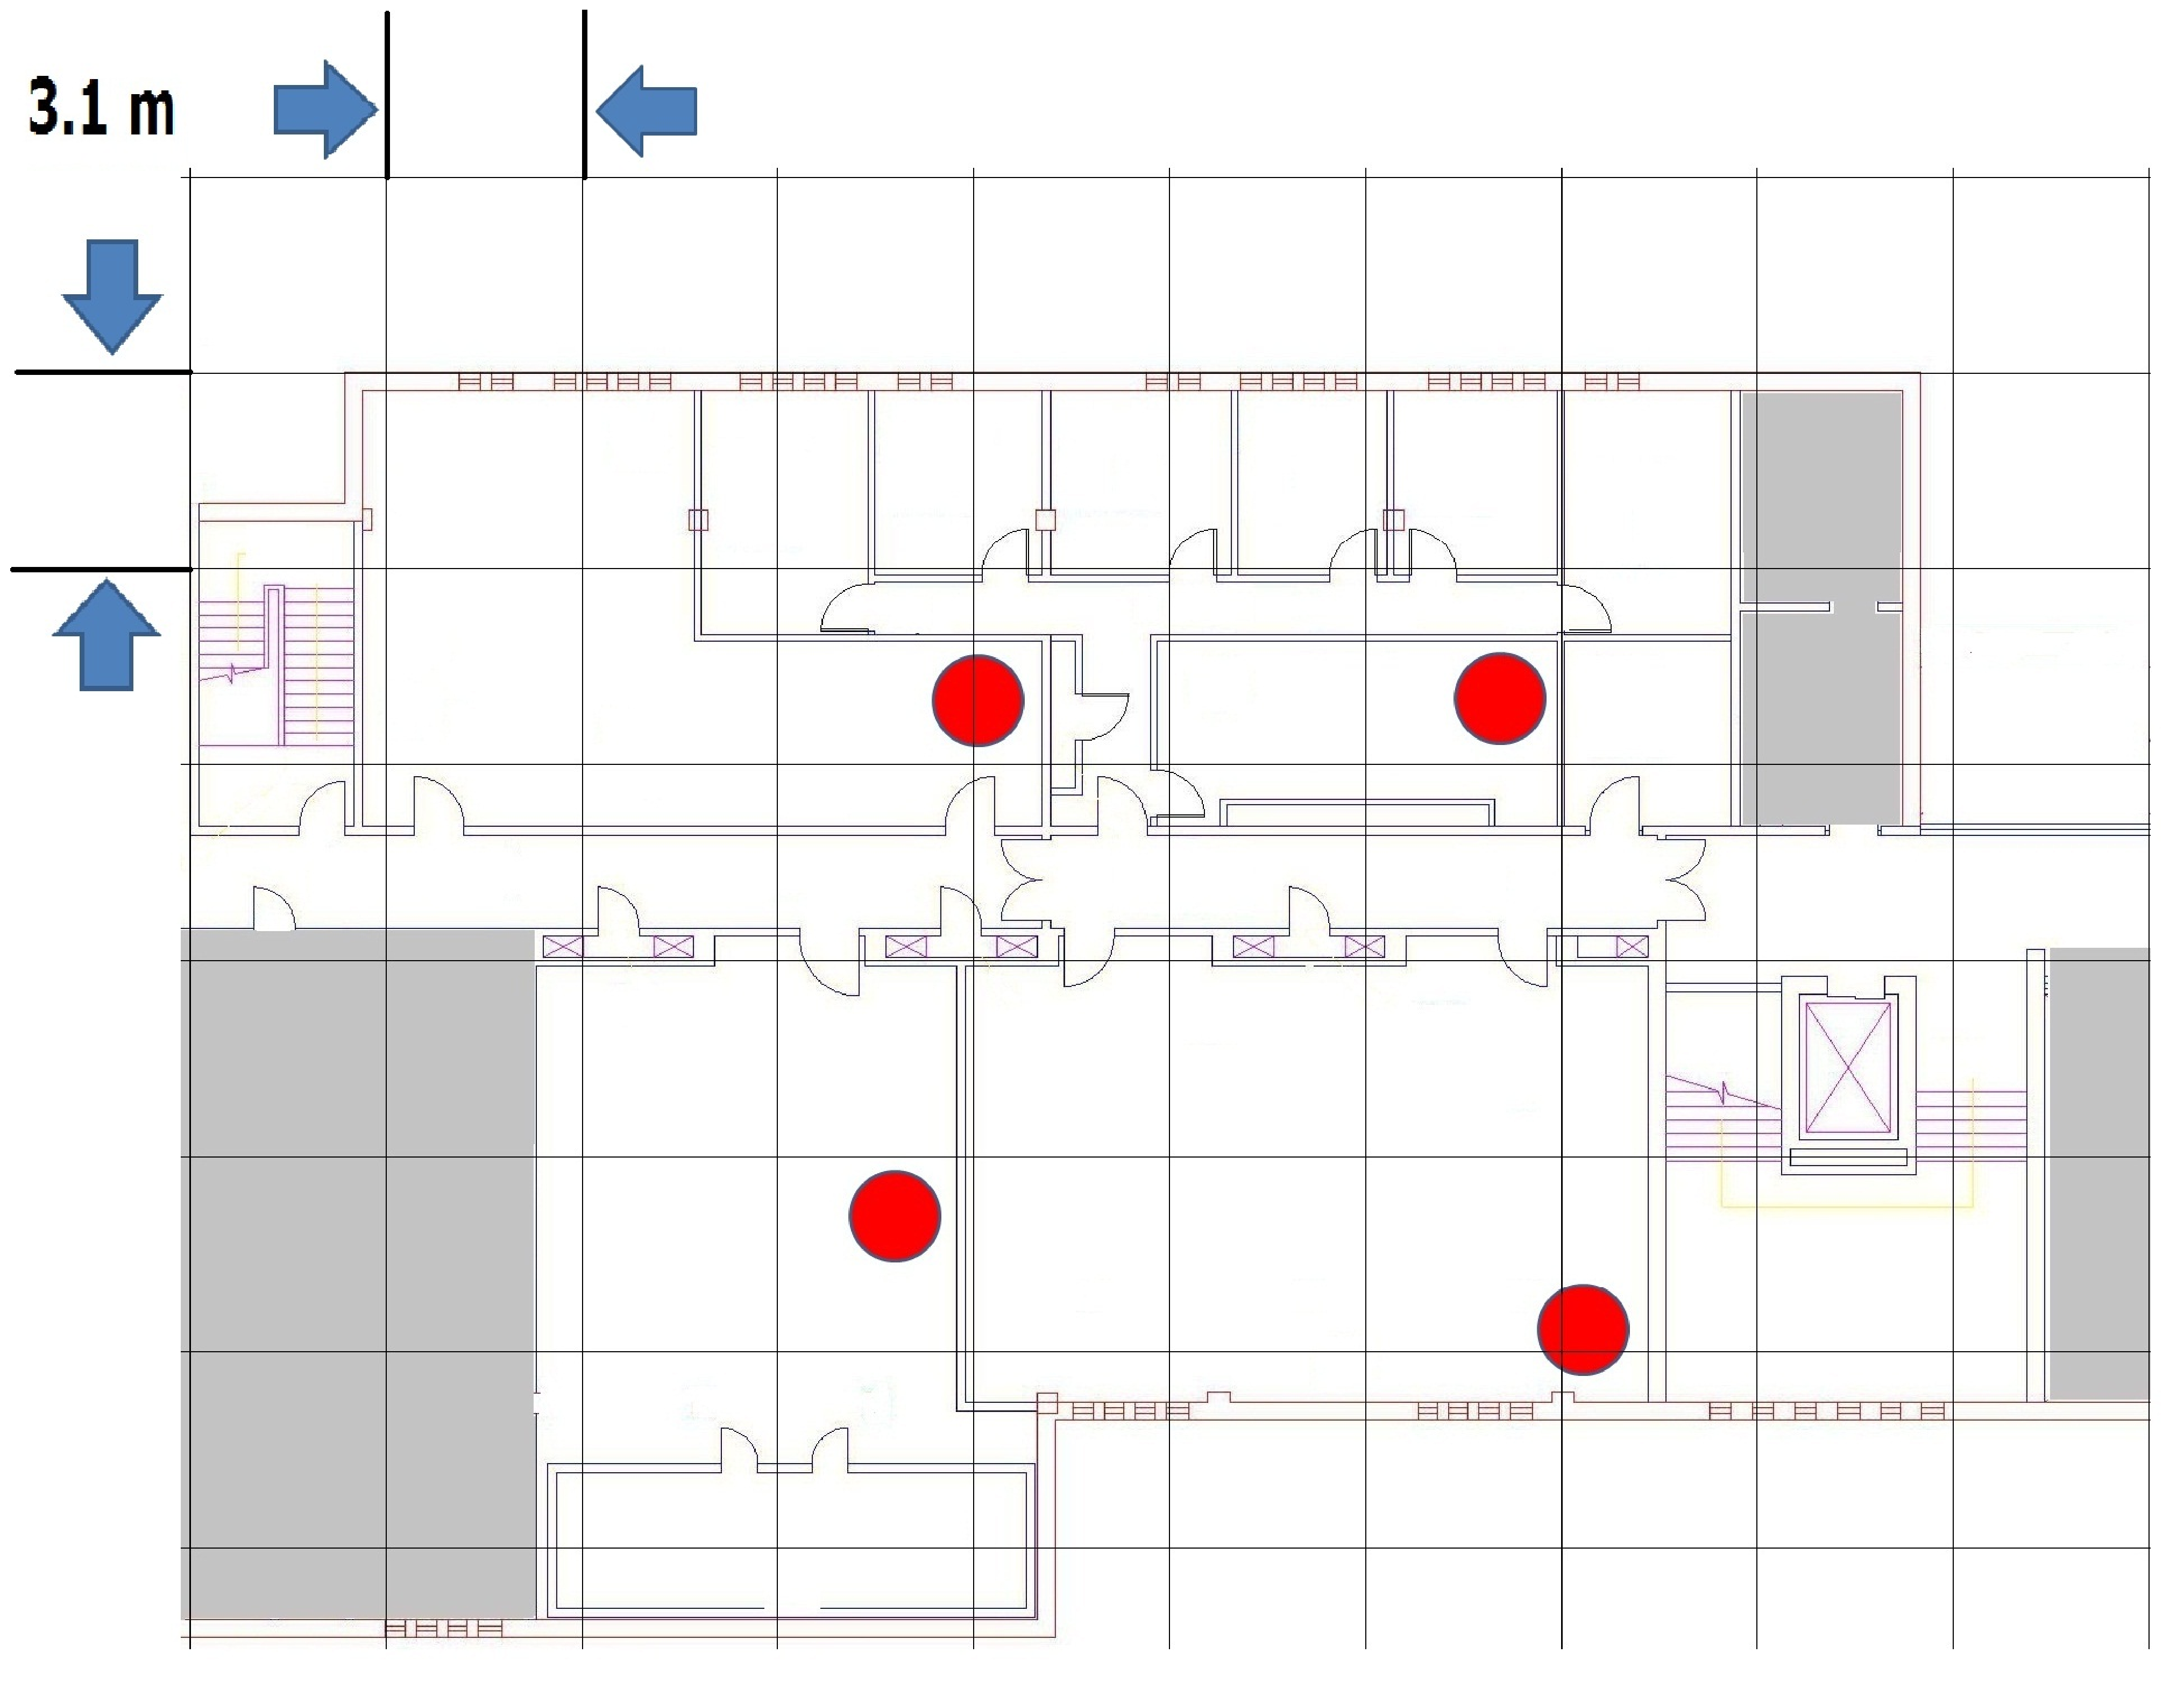
\epsfig{file=Figs4Paper/CSD/CSD-Map1.eps, height=1.5in, width=2.5in}
%   \caption{Map of the CS Dept Building where experiments were conducted}
%   \label{fig:csdbuilding}
% \end{figure}

Given a real-time received signal vector ${\bf {s}}^{(obs)}$, we can now find the location with the highest probability. We do this by first finding the probability for each (location, power-level) pair and then marginalizing over the power-levels. Thus the estimated location index is given by $j^{*}$ where
\begin{align}
j^{*} = max_{j} \sum_{k} P({x_{j}} = 1, {z_{k}} = 1 | {\bf {s}}^{(obs)}) 
\end{align}

\section{Experiment Methodology}
\label{sec:experimentmethodology}

In this section, we describe our methodology for doing the experiments. We start with a description of our system setup. This is followed by an overview of the components of our sniffer devices. We then present details about the two testbeds where we conducted our experiments. Finally we round up this section by discussing the data collection process.

\subsection{System Setup}
\label{subsec:systemsetup}

As mentioned briefly in Section 1.1, our system architecture is along the lines of an infrastructure-based model of location-determination systems. Our system has two main components: stationary sniffer devices in the target space and a centralized server running the GEM algorithm. Sniffers provide overlapping coverage of the target area ( similar to how APs are typically deployed inside buildings ). The server notifies the sniffers about the mac-id of the target device, the channel number and the listening period. The sniffers then record the signal strength of all packets received that match the server's query. The recorded information is sent to the backed server which makes a location estimation using the GEM algorithm.

In our current prototype, the server communicates with the sniffer devices using the pre-existing in-building power-line ethernet LAN. In the future, our sniffers functionality might be integrated directly into the WLAN APs of a production network. Enterprise APs usually have a centralized controller which can serve as our localization engine. This makes our architecture particularly interesting.

\subsection{Sniffer Information}
\label{subsec:snifferinformation}

Our sniffer devices are responsible for capturing wireless transmissions made by a Tx-client. We use soekris-net4801 boards as our sniffer
devices with atheros-based cm9 cards for wireless captures. Our sniffers are running Pyramid Linux (version 2.6.16-metrix) and we use the default
MadWiFi driver which comes with this distribution (0.9.4.5 : svn 1485). 

To capture packets we use the Tcpdump software (version 4.0.0 libpcap version 0.9.8) To obtain signal strength information, the MadWiFi driver allows a
monitor mode interface to be created and configured with RadioTap header support. From the radio-tap header we can extract the
Received Signal strength of each packet received by the sniffer. We verified that the MadWifi driver had a fixed noise-floor in each of our
cm9 cards (-95 dbm). In fact the received signal strength of a frame reported by the MadWiFi driver is actually the SNR value (in db) obtained after subtracting the noise-floor from the raw signal strength value. We work directly with the RSSI value (in db) as reported by the driver.

\begin{figure*}
	\centering
		\subfloat[CEWIT]{\includegraphics[height=1.5in, width=2.5in]{Figs4Paper/CEWIT/PowerPlot4Paper_CEWIT/PwrLvlPlot_cewit.eps}}
		\subfloat[CSD]{\includegraphics[height=1.5in, width=2.5in]{Figs4Paper/CSD/PowerPlot4Paper_CSD/PwrLvlPlot_csd.eps}}
	\caption{Number of power levels v/s Avg Error distance}
	\label{fig:powerlevelsvserrordistance}
\end{figure*}

\subsection{Testbed Details}
\label{subsec:testbeddetails}

We use two different testbeds to Experimentally validate our technique. The first (Fig 4), henceforth called CEWIT, is a large research and educational facility with a dimension of 65 $\times$ 50  meter square. The L-shaped floor comprises of several obstructions in the form of concrete walls, glass metal doors, server-rack cabinets housing a host of equipment gear etc. The second, henceforth called CSD, is a portion of the building housing Stony Brook University's Computer Science building. This rectangular-shaped floor has a dimension of 20 $\times$ 30 meter square and also contains several obstructions, including concrete walls, wooden partitions etc. Both these testbeds had a continuous flux of people moving around in the building while the experiments were conducted.

\subsection{Data Collection Methodology}
\label{subsec:datacollectionmethodology}

We perform our experiments with 4 different wireless devices - an android phone, an iphone, a dell laptop and a dell netbook. Our localization is performed on a discretized grid of the target space. The CEWIT testbed is discretized into 45 distinct locations roughly every 5.5 meters. The CSD testbed is divided into 27 distinct locations roughly every 3.3 meters. As part of our location estimation effort,  for each of the above four devices we transmit 200 ping packets from every distinct location of the corresponding testbed. This is typically done by having a user hold the mobile device and walk across the floor of the building briefly stopping at each marked location to transmit 200 ping packets. The ground truth is noted at each location before moving on to the new location. Note that the ground truth information is used only for evaluation of the localization error and is not supplied to GEM for training. Each ping packet is separated uniformly apart at a rate of 1 per second. The RSS vector for each transmission is composed of the signal strength value recorded by each individual sniffer. The sequence number in the ping packet is used to form this vector of RSS values from each transmission. Thus, from each distinct location on the map and for each device type, we have a set of 200 RSS tuples. This comprises our entire data set that we use in this paper. Experiments on RADAR [x] and Probabilistic [y] described later in this paper use a subset of this dataset for building the RF signal map and the remainder data for calculating localization error.

In the CEWIT testbed, we have six sniffer devices. The CSD testbed has four sniffers. The circular-dots in figure x and y show the sniffer positions in each separate testbed. As mentioned in Section [p and q] we assume knowledge of the sniffer positions in the map and use this information to calculate the signal strength values given by the indoor radio propagation model (Section a). These values are used to initialize our algorithm as explained in Section [p] .

\section{Evaluation}
\label{sec:evaluation}

\begin{figure}
\centering
  \epsfig{file=Figs4Paper/CEWIT/LearningSize4Paper_CEWIT/LearningSetSize_cewit.eps, height=1.5in, width=2.5in}
  \caption{Learning Set Size v/s Error distance on CEWIT Dataset}
  \label{fig:learningsetsizevserrordistance}
\end{figure}

\begin{figure*}
	\centering
	      \subfloat[CEWIT]{\includegraphics[height=1.5in, width=2.5in]{Figs4Paper/CEWIT/Baseline4Paper_CEWIT/BaselineComparisonsMedianError_cewit.eps}}
	      \subfloat[CSD]{\includegraphics[height=1.5in, width=2.5in]
	      {Figs4Paper/CSD/Baseline4Paper_CSD/BaselineComparisonsMedianError_csd.eps}}
	\caption{Baseline Comparisons}
	\label{fig:baselinecomparisons}
\end{figure*}

\begin{figure*}
\begin{minipage}{0.5\textwidth}
	{\centering
	  \subfloat[Probabilistic]{\includegraphics[width=0.5\textwidth]{Figs4Paper/CEWIT/HRComparisons4Paper_CEWIT/HRComparisonsMedianError_Probabilistic_cewit.eps}}
	  \subfloat[RADAR]{\includegraphics[width=0.5\textwidth]{Figs4Paper/CEWIT/HRComparisons4Paper_CEWIT/HRComparisonsMedianError_RADAR_cewit.eps}}
	\caption{Comparisons on the CEWIT Testbed}
	\label{fig:HR_on_cewittestbed}
	}
\end{minipage}\quad
\begin{minipage}{0.5\textwidth}
	{\centering
		\subfloat[Probabilistic]{\includegraphics[width=0.5\textwidth]{Figs4Paper/CSD/HRComparisons4Paper_CSD/HRComparisonsMedianError_Probabilistic_csd.eps}}
		\subfloat[RADAR]{\includegraphics[width=0.5\textwidth]{Figs4Paper/CSD/HRComparisons4Paper_CSD/HRComparisonsMedianError_RADAR_csd.eps}}
	\caption{Comparisons on the CSD Testbed}
	\label{fig:HR_on_csdtestbed}
	}
\end{minipage}
\end{figure*}

We implement our algorithm based on the EM algorithm and collection
accuracy estimates on the data sets collected from both testbeds.\\ 

We generate plots for the following experiments:

\begin{enumerate}
{\bf \item Number of power-levels used for EM: }\\
This experiment serves to give us the value of k (the number of
power-levels) that we should use in our algorithm.

{\bf \item Size of the learning set:}\\
This experiment shows how the average error distance varies as a
function of the learning set size.

{\bf \item Baseline Comparisons:}\\
This set of experiments is used to compare our technique with a baseline
Model-based scheme, both of which be applied on the fine-grained
discretized target space.

{\bf \item Comparisons with schemes that build RF signal maps:}\\
Here we compare our technique with two schemes that use an {\it offline
phase} to first build an RF signal map of the target space. 

{\bf \item Mobility-related experiments:}\\
These experiments show how the mobility of the Tx-client effects the
accuracy of our algorithm.

\end{enumerate}

\subsection{Avg. error distance v/s Number of power-levels used for EM}
\label{subsec:avgerrordistancevsnumberofpowerlevelsusedforEM}



We see that the avg. error distance does not vary much after we use k=45
in our EM algorithm. The subsequent plots shown here have been generated
using k = 45 in the algorithm. 

\subsection{Learning Set Size}
\label{subsec:learningsetsize}

As mentioned in Section \ref{subsec:datacollectionmethodology} for every device, we
have 200 RSS vectors for each location on the map. Figure
\ref{fig:learningsetsizevserrordistance} shows how the Average Error varies for
different sizes of the learning set i.e if we use m samples to learn the
parameters of the model which we subsequently use to localize the
remaining (200 - m) samples for each location. We see that the average error reaches almost
hits a plateau after 50 learning samples. The subsequent plots shown here
have been generated using 50 RSS samples to learn the model parameters. We
then use these parameters to localize the remaining 150 samples for each location.

\begin{figure*}
	\centering
		\subfloat[CEWIT]{\includegraphics[height=1.5in, width=2.5in]{Figs4Paper/CEWIT/MobilityPlot4paper_CEWIT/Mobility_cewit.eps}}
		\subfloat[CSD]{\includegraphics[height=1.5in, width=2.5in]{Figs4Paper/CSD/MobilityPlot4paper_CSD/Mobility_csd.eps}}
	\caption{Mobility}
	\label{fig:mobility}
\end{figure*}

\subsection{Baseline Comparison}
\label{subsec:baselinecomparison}


Here we compare our technique with a baseline Model-based technique that
can be applied on the fine-grained discretized target space shown in fig
\ref{fig:cewitbuilding} (a) and \ref{fig:csdbuilding} (a) . The
log-distance path loss (LDPL) mentioned in Section
\label{subsec:radiopropagation} is used to predict the RSS at each
square vertex that lies inside the target-space. The baseline uses directly
uses these values with NNSS as the metric to compare the multiple locations on the map 
and pick the one that best matches the observed signal strength vector.
Our algorithm instead uses these values to initialize our algorithm.
For each device, our algorithm uses 50 RSS samples from each location to
update the parameters of our model.  The new parameters are then used to
localize the remaining 150 RSS samples from each location.

\subsubsection{CEWIT-Dataset Baseline Comparisons}
\label{subsubsec:cewitdatasetbaselinecomparisons}

\subsubsection{CSD-Dataset Baseline Comparisons}
\label{subsubsec:csddatasetbaselinecomparisons}


We clearly see that we score over the baseline algorithm for all four
devices across both the testbeds.

\subsection{Comparisons with schemes that build RF signal maps}
\label{subsec:comparisonswithschemesthatbuildrfsignalmaps}

We next compare our technique with two schemes that need to have a
training phase to build an RF signal map first. Section
\label{sec:testbeddetails} explains why we use a coarser
granularity as shown in Figure \ref{fig:cewitbuilding} (b) and
\ref{fig:csdbuilding} (b) to build our signal map.

One of our comparison schemes is deterministic and is based on RADAR
\cite{Bahl00radar:an}. We use NNSS as the metric to identify the location
which best matches the observed signal strength vector. The other is a
probabilistic scheme on the lines of \cite{Haeberlen:2004:PRL:1023720.1023728}. Given a
location and a sniffer, signal intensity is modelled as a Gaussian
distribution based on the training data. We then use a MLE approach to
give a location fix for a target RSS fingerprint.

\subsubsection{CEWIT-Dataset Comparisons}
\label{subsubsec:cewitdatasetcomparisons}

{\bf {Trainer-Dell Laptop \\
			Test-Dell Laptop, Dell Netbook, Android, Iphone}}


\subsubsection{CSD-Dataset Comparisons}
\label{subsubsec:csddatasetcomparisons}


{\bf {Trainer-Android \\
	Test-Android, Iphone, Laptop, Netbook}}


We see that our algorithm performs at-par with state-of-the-art
RF-signal-map based techniques especially in cased where the target
device is different from the trained device. That is what makes our
technique particularly suitable for server-based localization where we
do not know the device type of the client being localized.

\subsection{Mobility}
\label{subsec:mobility}

This section shows how the mobility of a client can effect the location
estimates made by our algorithm.

In our first experiment, the client makes 2 random walks through the
building (i.e a random walk through 50 locations on the CEWIT testbed /
30 locations on the CS Dept testbed) transmitting just a single packet from each
location.

In the second experiment, the client makes 10 random walk through the
building again transmitting just a single packet from each location. 

In the last experiment, the client makes 50 random walk through the 
building again transmitting just a single packet from each location. 

\subsubsection{CEWIT-Dataset Mobility}
\label{subsubsec:cewitdatasetmobility}


\subsubsection{CSD-Dataset Mobility}
\label{subsubsec:csddatasetmobility}


We see that mobility progressively improves the localization accuracy of
our technique. More importantly, in 10 random walks itself we get pretty close
to the accuracy estimates obtained from 50 random walks. 

\section{Conclusions}
\label{sec:conclusions}

In this work, we have developed a server-side technique to localize a
wireless client in an indoor environment based on the signal strength
parameter of its transmitted packets. We developed a learning-based
algorithm that can learn the parameters of the model
dynamically from packets captured by the stationary sniffers / APs
inside the building. By using dynamic packet captures for parameter
estimation, we can provide location estimates which are much more robust in the face of time
varying phenomena like movement of people inside the building, opening
closing of doors etc. Moreover, this technique can be used on a host of
heterogeneous devices operating at different power levels. 

We do not have an explicit {\it training} phase in our technique.
Infact, we showed that we can achieve accuracy that is at par with state-of-the-art
techniques that use training to build RF-signal maps first. Thus,
our technique not only eliminates the intensive time-consuming (often manual) training phase
but also makes our technique scalable for large target spaces.

\section{Placeholder. BibRef. (To Remove)}
Haeberlen04 \cite{Haeberlen:2004:PRL:1023720.1023728},
Gwon04 \cite{Gwon:2004:ECC:1023783.1023786},
Elnahraway04 \cite{Elnahraway:2004:LLU:1031495.1031537},
Moraes06 \cite{Moraes:2006:CWL:1164783.1164799},
Youssef08 \cite{Youssef:2008:HLD:1399551.1399558},
Ferris07 \cite{Ferris:2007:WUG:1625275.1625675},
Berna03 \cite{Berna:2003:LAL:1630659.1630885},
Lim10 \cite{Lim:2010:ZIL:1741400.1741464},
Tsui09 \cite{Tsui:2009:ULS:1741410.1741596},
Chintalapudi10 \cite{Chintalapudi:2010:ILW:1859995.1860016},
Ladd02 \cite{Ladd:2002:RLS:570645.570674},
Youssef03 \cite{Youssef:2003:WLD:826025.826335},
Tao03 \cite{Tao:2003:WLL:941311.941314},
Krishnan04 \cite{Krishnan04asystem},
Borman \cite{Borman_theexpectation},
Bilmes97 \cite{Bilmes97agentle},
Roos02 \cite{Roos},
Elnahrawy \cite{Elnahrawy05bayesianindoor},
Bahl00 \cite{Bahl00radar:an},
Molkdar91 \cite{Molkdar},
Bishop \cite{Bishop:2006:PRM:1162264},
Reynolds \cite{Reynolds}

% The following two commands are all you need in the
% initial runs of your .tex file to
% produce the bibliography for the citations in your paper.
\bibliographystyle{abbrv}
\bibliography{sigproc}  % sigproc.bib is the name of the Bibliography in this case
% You must have a proper ".bib" file
%  and remember to run:
% latex bibtex latex latex
% to resolve all references
%
% ACM needs 'a single self-contained file'!
%

\end{document}  % This is where a 'short' article might terminate
